\section{Auswertung}
\label{sec:Auswertung}
\subsection{Durchbiegung des runden Stabes}
Der runde Stab weißt folgende Daten und Abmessungen auf
\begin{align*}
    \text{Länge: } l&=\qty{0,589(0.001)}{\meter},\\
    \text{Durchmesser: } d&=\qty{1,0(0,1)e-3}{\meter},\\
    \text{Masse: } m&=\qty{0,4116(0.0001)}{\kilo\gram}.
\end{align*}
Daraus ergibt sich für das Volumen und die Dichte 
\begin{align*}
    V&=\qty{4.6(0.05)e-5}{\meter\cubed},\\
    \rho&=\qty{8.9(0.09)e3}{\kilo\gram\per\meter\cubed}.
\end{align*}
Die Fehler werden über Pythons Applikation \textit{SciPy} via der Gaußschen 
Fehlerforpflanzung berechnet
\begin{equation}
    \increment f=\sqrt{\sum_{k=1}^{n}\biggl(\frac{\partial f}{\partial x_\text{k}}\biggr)^2(\increment x_\text{k})^2}\,.
    \label{eq:gauss}
    \end{equation}
Dabei ist $f$ die zur Berechnung der Größe gegebene Formel und $x_k$ dessen Argumente.
$\increment x_k$ ist der jeweilige Fehler der einzelnen Argumente.\\ 
Mittelwerte, Standardabweichungen und sonstige Fehler werden für diesen Versuch alle mit Python bzw. 
numeric python berechnet. \noindent 
Der Wert der Dichte entspricht dem Literaturwert für Kupfer. Hier Referenz einfügen!!
Auch das äußere Erscheinungsbild deutet auf Kupfer hin.
\subsubsection{Einseitige Einspannung}
Für die einseitige Einspannung des Stabes ergeben sich die in \autoref{tab:rund1} 
aufgeführten Messwerte. Der Stab ist bei $L=\qty{51,5}{\centi\meter}$ eingespannt.
\begin{table}
    \centering
    \label{tab:rund1}
    \caption{Abstand zur Einspannung, Auslenkung mit und ohne Gewicht sowie deren Differenz.}
    \begin{tblr}{colspec={c c c c||c c c c}}
        \toprule
        $x$\ /\ cm & $D_0$\ /\ mm & $D_\text{Gewicht}$\ /\ mm & $\increment D$&
        $x$\ /\ cm & $D_0$\ /\ mm & $D_\text{Gewicht}$\ /\ mm & $\increment D$\\
        \midrule
        50 & 5.71 & 2.47 & 3.24 & 26 & 7.10 & 5.91 & 1.19\\
        47 & 5.90 & 3.06 & 2.84 & 23 & 7.24 & 6.28 & 0.96\\
        44 & 6.29 & 4.40 & 1.89 & 20 & 7.35 & 6.58 & 0.77\\
        41 & 6.38 & 3.92 & 2.46 & 17 & 7.47 & 6.89 & 0.58\\
        38 & 6.53 & 4.32 & 2.21 & 14 & 7.57 & 7.17 & 0.40\\
        35 & 6.76 & 4.81 & 1.95 & 11 & 7.69 & 7.41 & 0.28\\
        32 & 6.90 & 5.17 & 1.73 & 08  & 7.78 & 7.61 & 0.17\\
        29 & 7.00 & 5.55 & 1.45 & 05  & 7.82 & 7.74 & 0.08\\
        \bottomrule
    \end{tblr}
\end{table}
Es sollen nun die Elastizitätsmodule der Stäbe bestimmt werden. Dafür wird jeweils eine lineare Regression der Form
$l(x)=ax+b$ durch die Messwerte gelegt, welche nach Gleichung \eqref{eq:polynom1} lineariesiert werden. Der Vorfaktor 
$\sfrac{F}{2EI}$ des Polynoms $Lx^2-\sfrac{x^3}{3}$ ist dabei die Steigung der Ausgleichsgeraden. Da $F$ und $I$ 
aus den gegebenen Größen direkt berechnet werden können, kann $a=\sfrac{F}{2EI}$ direkt nach dem Elastizitätsmodul $E$
umgestellt werden. Das Flächenträgheitsmoment $I$ wird über $I=\sfrac{\pi d^4}{64}$ berechnet REFERENZ!!. In 
\autoref{fig:plota} sind die Messwerte der ersten Messreihe sowie die lineare Regression zu sehen. Die angehangene 
Masse beträgt $m=\qty{0,5}{\kilo\gram}$
\begin{figure}[H]
    \centering
    \label{fig:plota}
    \caption{Messwerte des einseitig eingespannten runden Stabes und deren lineare Regression.}
    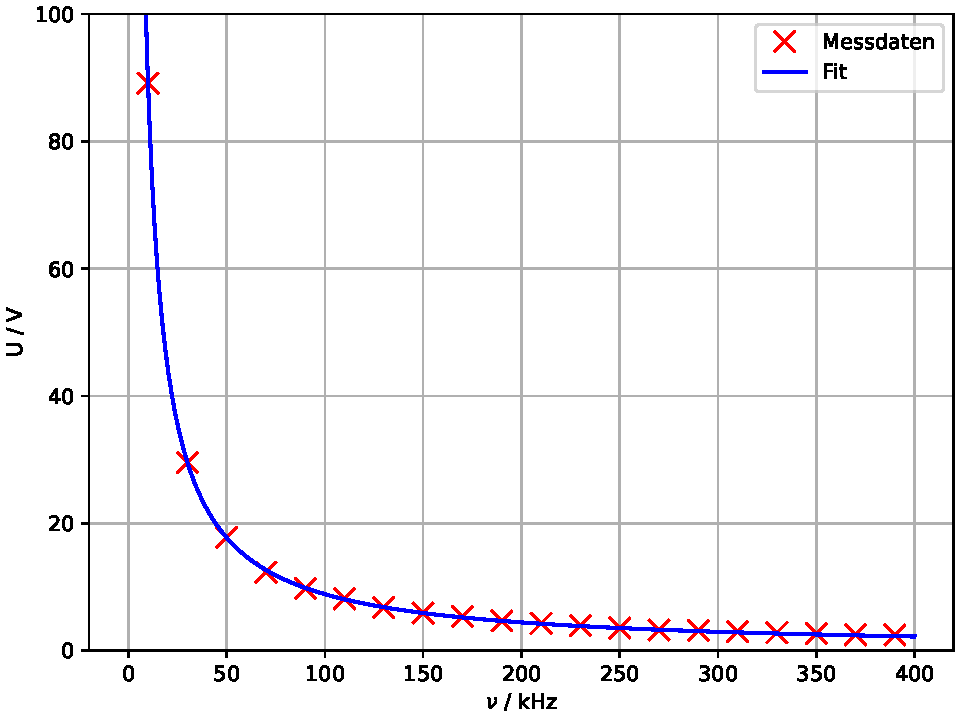
\includegraphics[width=\textwidth]{build/plota.pdf}
\end{figure}
Für die Koeffizienten ergeben sich mit \textit{Python} die Werte
\begin{align*}
    a&=\qty{3,4(0,19)e-2}{\per\meter\squared},\\
    b&=\qty{1,4(0,9)e-4}{\meter}.
\end{align*}
Der Elastizitätsmodul berechnet sich über
\begin{align*}
E&=\frac{F}{2aI}
\intertext{mit}
F&=mg=\qty{0,5}{\kilo\gram}\cdot\qty{9,806}{\meter\per\second\squared} \text{ und } I=\qt{4,91e-10}{\meter\tothe{4}}
\intertext{zu}
E_1&=\qty{146(8,2)}{\giga\pascal}\,.
\end{align*}
\subsubsection{Beideitig Einspannung}
Zur beidseitigen Einspannung des runden Stabes ergeben sich die in \autoref{tab:rund2} aufgeführten Messwerte.
\begin{table}
    \centering
    \label{tab:rund2}
    \caption{Messwerte der Durchbiegung eines runden Stabes links und rechts der Mitte mit und ohne Gewicht.}
    \begin{tblr}{colspec={c c c c c c c c}}
        \toprule
        $x_\text{l}$\ /\ cm & $x_\text{r}$\ /\ cm  & $D_{0\text{l}}$\ /\ mm & $D_\text{Gewicht,l}$\ /\ mm &
        $D_{0\text{r}}$\ /\ mm & $D_\text{Gewicht,r}$\ /\ mm & $\increment D_\text{l}$ & $\increment D_\text{l}$ \\
        \midrule
        31 & 24 & 7.16 & 7.61 & 6.89 & 7.36 & 0.27 & 0.25\\
        32 & 23 & 7.17 & 7.60 & 6.93 & 7.39 & 0.24 & 0.20\\
        33 & 22 & 7.18 & 7.63 & 6.83 & 7.40 & 0.35 & 0.23\\
        34 & 21 & 7.15 & 7.65 & 6.89 & 7.44 & 0.26 & 0.21\\
        35 & 20 & 7.14 & 7.64 & 6.88 & 7.44 & 0.26 & 0.20\\
        37 & 18 & 7.14 & 7.65 & 6.89 & 7.46 & 0.25 & 0.19\\
        39 & 16 & 7.13 & 7.72 & 6.90 & 7.68 & 0.23 & 0.04\\
        41 & 14 & 7.11 & 7.75 & 6.89 & 7.61 & 0.22 & 0.14\\
        43 & 12 & 7.08 & 7.77 & 6.89 & 7.69 & 0.19 & 0.08\\
        45 & 10 & 7.02 & 7.82 & 6.86 & 7.74 & 0.16 & 0.08\\
        47 & 08 & 7.06 & 7.83 & 6.93 & 7.77 & 0.13 & 0.06\\
        \bottomrule
    \end{tblr}
\end{table}
Aus diesen Messwerten lassen sich zwei Plots erstellen und damit zwei mal der Elastizitätsmodul bestimmen.
\autoref{fig:plotb} zeigt die lineare Regression sowie die Messdaten der rechten Seite, \autoref{fig:plotc} 
die der linken. Für die Messwerte der rechten Seite ($x\leq\sfrac{L}{2}$) wird die $x-Skala$ nach Formel 
\eqref{eq:rechts} skaliert, für die linke Seite nach Formel \eqref{eq:links}.
\begin{figure}[H]
    \centering
    \label{fig:plotb}
    \caption{Messwerte sowie die lineare Regression der Durchbiegung des beidseitig eingespannten runden Stabes rechtsseitig.}
    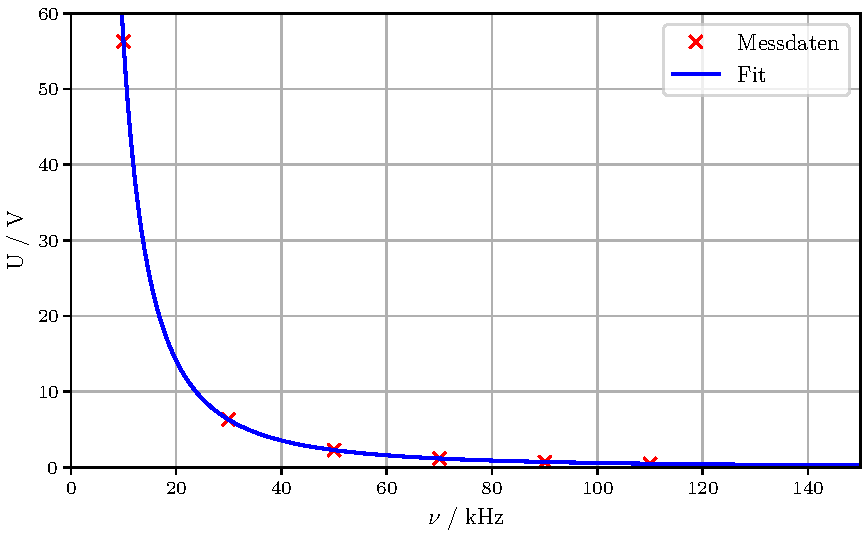
\includegraphics[width=\textwidth]{build/plotb.pdf}
\end{figure}
\begin{figure}[H]
    \centering
    \label{fig:plotc}
    \caption{Messwerte sowie die lineare Regression der Durchbiegung des beidseitig eingespannten runden Stabes linksseitig.}
    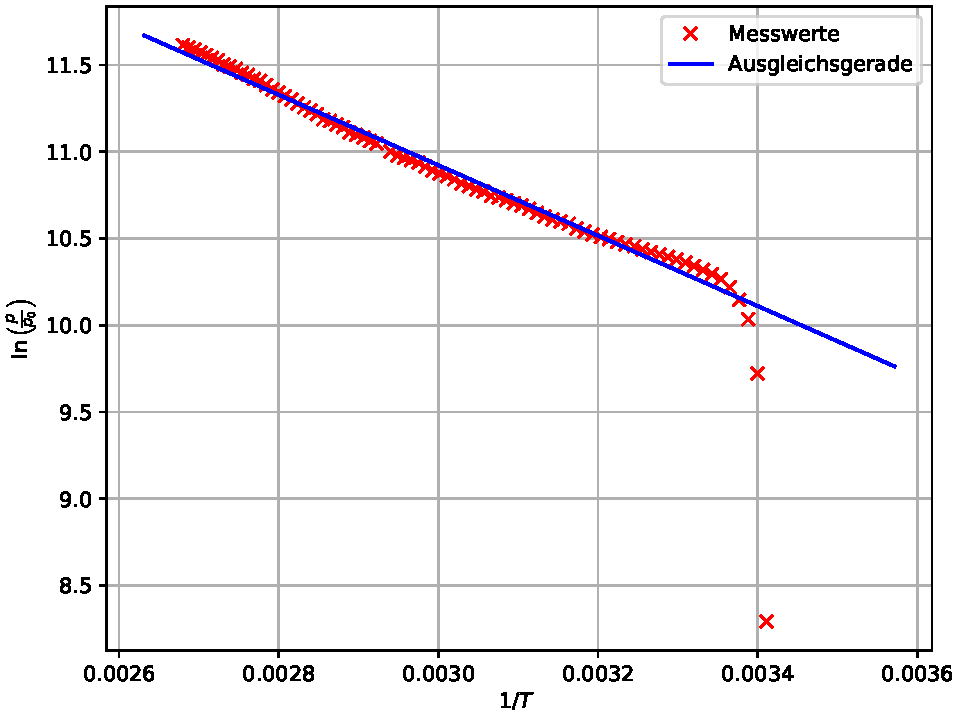
\includegraphics[width=\textwidth]{build/plotc.pdf}
\end{figure}

Es ergeben sich die Koeffizienten 
\begin{align*}
    a&=\qty{2(0.4)e-3}{\per\meter\squared}\,,\\
    b&=\qty{-1.1(0.6)e-4}{\meter}\,.
\end{align*}
Über das gleiche Vorgehen wie bei einseitiger Einspannung ergibt sich für den Elastizitätsmodul

#Koeffizienten linke Seite(größer L/2)
a = 0.00161 ± 0.00029
b = 0.00008 ± 0.00003
#Koeffizienten eckiger Stab einseitig
Volumen quadratischer Stab:  (6.00+/-0.06)e-05 m^3
Dichte quadratischer Stab:  (8.93+/-0.09)e+03 kg/m^3
a = 0.02551 ± 0.00027
b = 0.00004 ± 0.00001